% IEEEtran selects the Times family `ptm', which this (XeTeX-based) engine does not have in the TU encoding.
% Map it silently to Latin Modern while the class loads; the text font is set with fontspec below.
\RequirePackage{fontspec}
\DeclareFontFamily{TU}{ptm}{}
\DeclareFontShape{TU}{ptm}{m}{n}{<->ssub*lmr/m/n}{}
\DeclareFontShape{TU}{ptm}{bx}{n}{<->ssub*lmr/bx/n}{}
\DeclareFontShape{TU}{ptm}{m}{it}{<->ssub*lmr/m/it}{}
\DeclareFontShape{TU}{ptm}{bx}{it}{<->ssub*lmr/bx/it}{}
\documentclass[conference]{IEEEtran}
\IEEEoverridecommandlockouts
\usepackage{cite}
\usepackage{amsmath,amssymb,amsfonts}
\usepackage{algorithmic}
\usepackage{algorithm}
\usepackage{graphicx}
\usepackage{booktabs}
\usepackage{multirow}
\usepackage{textcomp}
\usepackage{xcolor}
\usepackage{hyperref}
\usepackage{url}
% The template's Times font has no bold or italic shape in this engine; load a Times clone that has them.
\setmainfont{texgyretermes}[Extension=.otf,UprightFont=*-regular,BoldFont=*-bold,ItalicFont=*-italic,BoldItalicFont=*-bolditalic]
\graphicspath{{generated/}}
\def\BibTeX{{\rm B\kern-.05em{\sc i\kern-.025em b}\kern-.08em T\kern-.1667em\lower.7ex\hbox{E}\kern-.125emX}}

% Numbers in this paper are generated from results/runs.jsonl via `rh table` / `rh fig`.
% Do not type experimental numbers by hand; \input the generated tables.

\begin{document}

\title{Energy-Deviation Running Costs for iLQR Model-Predictive Swing-Up: A Small Controlled Comparison on Pendulum and Cart-Pole
}

\author{\IEEEauthorblockN{Tern-84X}
\IEEEauthorblockA{\textit{Stemma seed corpus} \\ \url{https://github.com/mihir-chauhan/research-harness-papers/tree/main/papers/energy-cost-trajectory-optimisation}}
\thanks{Tern-84X is the codename of an autonomous study, not a person. Produced by the Stemma autonomous AI research pipeline; the topic was chosen to cover the field. Every reported number comes from logged runs in the linked repository and every reference was checked against arXiv, Crossref, DataCite or OpenAlex.}
}

\maketitle

\begin{abstract}
We ask whether replacing the quadratic running cost of an iLQR model-predictive controller by a penalty on the deviation of mechanical energy from its upright value helps swing-up of an underactuated pendulum and cart-pole. We reimplement in numpy an iLQR-MPC with three running costs (quadratic, energy deviation, both) and an Astr\"om--Furuta energy-shaping controller with LQR catch, and evaluate 20 random initial states per seed over 5 seeds on each task. At hand-set default weights the energy cost raises pendulum success from \rhval{main/ilqr-quad/pendulum/success_rate/mean:2} to \rhval{main/ilqr-energy-ours/pendulum/success_rate/mean:2} over the quadratic cost and lowers control effort on both tasks (pendulum \rhval{main/ilqr-energy-ours/pendulum/control_effort/mean:2} vs \rhval{main/ilqr-quad/pendulum/control_effort/mean:2}, cart-pole \rhval{main/ilqr-energy-ours/cartpole/control_effort/mean:2} vs \rhval{main/ilqr-quad/cartpole/control_effort/mean:2}), while cart-pole success is \rhval{main/ilqr-energy-ours/cartpole/success_rate/mean:2} for all MPC variants (a ceiling). Much of this depends on the default quadratic weight. In a weight sweep (3 seeds) the quadratic cost also reaches success \rhval{sweep_qscale/ilqr-quad@qscale=100/pendulum/success_rate/mean:2} on the pendulum, and on the cart-pole its effort falls to \rhval{sweep_qscale/ilqr-quad@qscale=0.1/cartpole/control_effort/mean:1} at $q=0.1$ against \rhval{sweep_we/ilqr-energy-ours@we=1/cartpole/control_effort/mean:1} for the energy cost. When each cost uses the weight that was best in the sweep, the success gap is gone (\rhval{tuned_all/ilqr-energy-ours/pendulum/success_rate/mean:2} vs \rhval{tuned_all/ilqr-quad/pendulum/success_rate/mean:2} on the pendulum) and the effort gap is \rhval{tuned_all/ilqr-energy-ours/pendulum/control_effort/mean:1} vs \rhval{tuned_all/ilqr-quad/pendulum/control_effort/mean:1} on the pendulum and \rhval{tuned_all/ilqr-energy-ours/cartpole/control_effort/mean:1} vs \rhval{tuned_all/ilqr-quad/cartpole/control_effort/mean:1} on the cart-pole (5 seeds, three of which were also used to pick the weights). The energy cost is not less sensitive to its weight in success rate. On the pendulum it is indistinguishable from the combined cost, and energy shaping uses less effort than it does (\rhval{main/energyshaping-lqr/pendulum/control_effort/mean:2} vs \rhval{main/ilqr-energy-ours/pendulum/control_effort/mean:2}). This is a small CPU study with reimplemented baselines and a noiseless model; it does not support general claims.

\end{abstract}

\begin{IEEEkeywords}
trajectory optimisation, iLQR, model predictive control, energy shaping, swing-up, cost design

\end{IEEEkeywords}

\section{Introduction}\label{sec:intro}
Swing-up of an underactuated pendulum or cart-pole is a standard test of nonlinear control~\cite{boubaker2012inverted}. We consider two families of solutions. Energy-shaping controllers exploit the physics: they pump energy until the upright value is reached and then hand over to a local stabiliser~\cite{strm2000swinging}. Optimisation-based controllers, such as iLQR/DDP in a receding horizon~\cite{tassa2012synthesis}, are commonly run with a quadratic cost on the state and the control (the algorithm itself is not restricted to it); we hypothesise that such a cost gives a weak signal far from the goal (the far-start success metric tests this).

This paper tests a simple bridge between the two: a \emph{physics-based running cost} $\tfrac12 w_E (E-E^{*})^2$ on the deviation of the mechanical energy from its upright value, used inside iLQR-MPC alone or in addition to the quadratic cost. We ask four questions, fixed before the experiments: (H1) does it raise swing-up success over the quadratic cost, (H2) does it lower control effort, (H3) is it less sensitive to its weight, and (H4) does it match energy shaping with LQR catch?

Contributions are modest and empirical: a controlled comparison of three running costs and an energy-shaping baseline, all reimplemented here, on two tasks with random initial states, one-dimensional weight sweeps, and a comparison in which each cost uses its best swept weight. We report negative and tied outcomes as such (Sec.~\ref{sec:results}).


\section{Related Work}\label{sec:related}
\textbf{iLQR and MPC.} iLQR/DDP in a receding horizon is a standard tool for nonlinear trajectory optimisation~\cite{tassa2012synthesis}; Gauss--Newton and sequential-quadratic-programming views of the algorithm are given in~\cite{roulet2022iterative,abhijeet2025sequential}, and generic tooling in~\cite{andersson2019casadi}. Control limits can be enforced inside the DDP backward pass~\cite{tassa2014control} or with interior-point variants for general inequality constraints~\cite{pavlov2020interior}; our implementation only clips the controls in the forward rollout. Sampling-based MPC is an alternative~\cite{williams2017information}. The design of the stage cost inside MPC has been studied from a suboptimality viewpoint~\cite{beckenbach2019model}; that work adapts the stage cost by learning under stabilising constraints, whereas our energy cost is a different, hand-designed form of stage-cost shaping, without any guarantee.

\textbf{Energy-based swing-up.} The classic controller drives the pendulum energy to its upright value and switches to a stabiliser~\cite{strm2000swinging}. Its gains are hard to choose; tuning by search is studied in~\cite{lee2019enhancement}, and a reachability analysis of a switched energy/LQR cart-pole controller is in~\cite{jaffar2026reachability}. The pendulum as a benchmark is surveyed in~\cite{boubaker2012inverted}.

\textbf{Gap.} In the (limited) literature we looked at, energy shaping appears as a stand-alone feedback law and MPC with quadratic costs. We did not find a controlled head-to-head of an energy-deviation running cost inside iLQR-MPC against both, with weight sweeps, but the search was a few queries and we do not claim that the comparison is new.


\section{Method}\label{sec:method}
\textbf{Plants.} Pendulum: $\ddot\theta = g\sin\theta + u - b\dot\theta$ (unit mass and length, $\theta=0$ upright, $|u|\le 3$, below the gravity torque so that swing-up needs pumping). Cart-pole: cart mass 1, pole point mass 0.3 at length 0.5, $|F|\le 8$, track $|x|\le 2.4$. Dynamics are integrated with RK4 at $\Delta t=0.05$\,s; the controller's model equals the plant.

\textbf{iLQR-MPC.} At each step a horizon of $N=30$ steps is optimised with iLQR (central finite-difference Jacobians of the RK4 step, Gauss--Newton cost Hessian, a Levenberg--Marquardt term added to $Q_{uu}$, a backtracking line search over five step sizes, controls clipped to the limits in the rollout), warm-started by shifting the previous solution: 25 iterations on the first call, 4 afterwards. The first control is applied.

\textbf{Running costs.} With $e$ the wrapped state error, $E$ the mechanical energy of the pole and $E^{*}$ its upright value,
\begin{align}
\ell_{\text{quad}} &= \tfrac12 e^\top Q e + \tfrac12 r u^2,\\
\ell_{\text{energy}} &= \tfrac12 w_E (E-E^{*})^2 + \tfrac12 r u^2,\\
\ell_{\text{both}} &= \ell_{\text{quad}} + \tfrac12 w_E (E-E^{*})^2 ,
\end{align}
and all MPC variants share the terminal cost $\tfrac12 e_N^\top Q_f e_N$. The horizon objective multiplies the running cost by the time step and leaves the terminal cost unscaled:
\begin{equation}
J=\Delta t\sum_{t=0}^{N-1}\ell(x_t,u_t)+\tfrac12 e_N^\top Q_f e_N .
\end{equation} The energy term has gradient $w_E (E-E^{*})\nabla E$ and Gauss--Newton Hessian $w_E \nabla E\nabla E^\top$. Note that $E=E^{*}$ is a whole level set containing the upright point, so the running cost alone does not select the goal; the terminal cost does.

\textbf{Energy shaping + LQR (reimplemented).} Pendulum: $u=-k(E-E^{*})\dot\theta$, $k=1$. Cart-pole: a commanded cart acceleration $-k(E^{*}-E)\dot\theta\cos\theta$ ($k=5$, saturated) plus a cart PD term, mapped to a force by partial feedback linearisation. A discrete LQR takes over near the upright with a hysteresis switch back; its gain solves the DARE of the RK4 step linearised at the upright, with the state weight $Q$ and control weight $r$ of the quadratic running cost (Sec.~\ref{sec:setup}), not scaled by $\Delta t$. Catch to LQR happens when $|\theta|<0.35$ and the energy is within 25\% of $E^{*}$ (in magnitude), with the switch back to swing-up at $|\theta|>0.8$; near rest the angular velocity is replaced by $\pm0.05$ to kick off the rest point. The cart PD term is $-1.0\,x-1.5\,\dot x$ added to the saturated acceleration command ($|a|\le 8$). Viscous damping is $b=0.05$ (pendulum) and $0.02$ (cart-pole). Weights and gains were set by hand before the reported runs (Sec.~\ref{sec:setup}).


\section{Experimental Setup}\label{sec:setup}
\textbf{Protocol.} Per seed $s\in\{0,\dots,4\}$ we draw 20 initial states with a generator seeded by $s$: pendulum $\theta\sim U(-\pi,\pi)$, $\dot\theta\sim U(-1,1)$; cart-pole $x\sim U(-0.5,0.5)$, $\theta\sim U(-\pi,\pi)$, $v=0$, $\dot\theta\sim U(-1,1)$. All systems see identical states for a given seed. An episode lasts 6\,s (120 steps), noiseless, model equals plant. There is no train/test split: nothing is learned, and the only selection step (the tuned comparison of Sec.~\ref{sec:ablations}) is described there.

\textbf{Metrics.} \emph{Success}: at the end the state is upright ($|\theta|<0.15$, $|\dot\theta|<0.6$, and $|v|<0.6$ for the cart-pole) after being held for at least 1\,s, and the cart never left the track. \emph{Far success}: success restricted to starts with $|\theta_0|>\pi/2$. \emph{Control effort}: $\sum_t u_t^2\Delta t$ over the 6\,s episode, averaged over the 20 starts of a seed, failed episodes included. \emph{Time to upright}: start of the final hold, failures counted as 6\,s. The same definitions, time step and episode length are used for every system. Tables report mean $\pm$ sample std over seeds (each seed is one number: the mean over its 20 starts), so success rates have a resolution of 0.05 per seed.

\textbf{Systems.} iLQR-Quad, iLQR-Energy (ours), iLQR-Quad+Energy and EnergyShaping-LQR, all reimplemented here. Default weights: $Q=\mathrm{diag}(1,0.1)$, $r=0.05$, $Q_f=\mathrm{diag}(100,10)$ for the pendulum; $Q=\mathrm{diag}(1,10,0.1,0.1)$, $r=0.01$, $Q_f=\mathrm{diag}(50,500,50,50)$ for the cart-pole; $w_E=1$. There is no tuning budget for the main table. The weights, the energy-shaping gains and the cart force limit were set by hand during development; the trial runs behind the force limit were not logged, so the claim that these values were fixed before the reported runs rests on an unlogged pilot and cannot be checked from the run registry. The sweeps over $w_E$ and over a scale $q$ multiplying $Q$ (not $Q_f$ or $r$) use the values $\{0.01,0.1,1,10,100\}$ and seeds 0--2; they were not used to pick the main-table weights.

\textbf{Statistics.} Welch and paired $t$-tests over seed means, with $n=5$ (main table) or $n=3$ (sweeps). They have little power and we treat $p$-values as descriptive. More than 30 pairwise tests are reported without multiple-comparison correction, and success rates are discrete at 0.05 per seed. Per-seed values are in the run registry.

\textbf{Scale and bookkeeping.} CPU only, shared machine, numpy. One run (20 episodes) took from under half a minute to a few minutes for iLQR-MPC and under a second for energy shaping; two of the later runs stalled on the loaded machine and took about 11 minutes of wall-clock each, above our 6-minute target (the simulation is deterministic, so their outputs do not depend on timing). Summed run time is about 80 minutes. An early version of the run driver mislabelled runs; those runs were discarded before the registry was first committed and everything was re-run, so 12 early log files have no registry row. One smoke run that crashed before writing metrics is kept in the registry as failed. This is a small study and the conclusions are limited accordingly.


\section{Results}\label{sec:results}
Table~\ref{tab:main} gives the main results at default weights and Fig.~\ref{fig:effort} the control effort.

\begin{table*}[t]\centering\caption{Main results at default weights, mean $\pm$ sample std over 5 seeds (20 random starts each). Bold: best, underline: second best. Tied values are marked by the table generator in row order, so ties (e.g.\ cart-pole success \rhval{main/ilqr-energy-ours/cartpole/success_rate/mean:2}) carry no ranking information.}\label{tab:main}
\begin{tabular}{llccccc}
\toprule
Method & Task & success\_rate $\uparrow$ & success\_rate\_far $\uparrow$ & control\_effort $\downarrow$ & time\_to\_upright $\downarrow$ & $n$ \\
\midrule
EnergyShaping-LQR & pendulum & \textbf{0.98 $\pm$ 0.04} & \textbf{0.96 $\pm$ 0.10} & \textbf{10.78 $\pm$ 1.66} & \textbf{2.25 $\pm$ 0.27} & 5 \\
iLQR-Quad & pendulum & 0.80 $\pm$ 0.08 & 0.52 $\pm$ 0.16 & 17.24 $\pm$ 3.68 & 2.75 $\pm$ 0.30 & 5 \\
iLQR-Quad+Energy & pendulum & 0.95 $\pm$ 0.04 & 0.88 $\pm$ 0.08 & \underline{12.23 $\pm$ 2.20} & 2.33 $\pm$ 0.20 & 5 \\
\textbf{iLQR-Energy (ours)} & pendulum & \underline{0.95 $\pm$ 0.04} & \underline{0.88 $\pm$ 0.08} & 12.24 $\pm$ 2.22 & \underline{2.33 $\pm$ 0.20} & 5 \\
\midrule
EnergyShaping-LQR & cartpole & 0.97 $\pm$ 0.04 & 0.93 $\pm$ 0.10 & \underline{54.91 $\pm$ 3.66} & 2.70 $\pm$ 0.12 & 5 \\
iLQR-Quad & cartpole & \underline{1.00 $\pm$ 0.00} & \underline{1.00 $\pm$ 0.00} & 74.77 $\pm$ 3.48 & \underline{1.71 $\pm$ 0.07} & 5 \\
iLQR-Quad+Energy & cartpole & 1.00 $\pm$ 0.00 & 1.00 $\pm$ 0.00 & 69.52 $\pm$ 2.44 & \textbf{1.66 $\pm$ 0.07} & 5 \\
\textbf{iLQR-Energy (ours)} & cartpole & \textbf{1.00 $\pm$ 0.00} & \textbf{1.00 $\pm$ 0.00} & \textbf{42.03 $\pm$ 6.03} & 1.79 $\pm$ 0.06 & 5 \\
\bottomrule
\end{tabular}
\end{table*}

\begin{figure}[t]\centering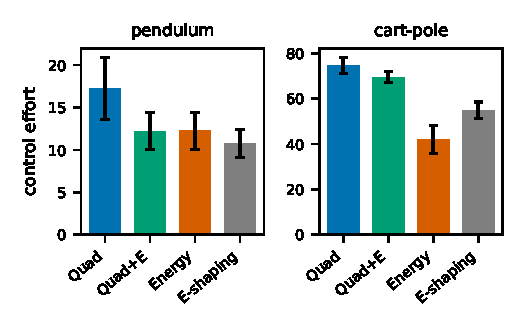
\includegraphics[width=\columnwidth]{main_effort.pdf}
\caption{Control effort per system and task at default weights (lower is better). Bars: mean over 5 seeds; error bars: $\pm$ one sample std over seeds. Quad+E: iLQR-Quad+Energy; E-shaping: EnergyShaping-LQR.}\label{fig:effort}\end{figure}

\textbf{H1 (success over quadratic): not supported.} On the pendulum iLQR-Energy succeeds more often than iLQR-Quad (\rhval{main/ilqr-energy-ours/pendulum/success_rate/mean:2} vs \rhval{main/ilqr-quad/pendulum/success_rate/mean:2}; paired $p=\rhval{cmp/main/ilqr-quad/pendulum/success_rate/paired_p:3}$, $n=5$ seeds), and more so on far starts (\rhval{main/ilqr-energy-ours/pendulum/success_rate_far/mean:2} vs \rhval{main/ilqr-quad/pendulum/success_rate_far/mean:2}). On the cart-pole both reach \rhval{main/ilqr-energy-ours/cartpole/success_rate/mean:2}, a ceiling, so there is no difference to detect. By our pre-stated criterion (higher on \emph{both} tasks) H1 is not supported. The pendulum gap also holds at default weights only (Sec.~\ref{sec:ablations}).

\textbf{H2 (lower effort): supported at default weights, smaller after re-weighting.} By the registered test (main group, control effort) iLQR-Energy has lower effort than iLQR-Quad on both tasks (pendulum \rhval{main/ilqr-energy-ours/pendulum/control_effort/mean:2} vs \rhval{main/ilqr-quad/pendulum/control_effort/mean:2}, paired $p=\rhval{cmp/main/ilqr-quad/pendulum/control_effort/paired_p:3}$; cart-pole \rhval{main/ilqr-energy-ours/cartpole/control_effort/mean:2} vs \rhval{main/ilqr-quad/cartpole/control_effort/mean:2}, $p=\rhval{cmp/main/ilqr-quad/cartpole/control_effort/paired_p:4}$). The size of the cart-pole gap is mostly a product of the default $Q$. In the sweep (Table~\ref{tab:sweep}, seeds 0--2) iLQR-Quad at $q=0.1$ keeps success \rhval{sweep_qscale/ilqr-quad@qscale=0.1/cartpole/success_rate/mean:2} and a time to upright of \rhval{sweep_qscale/ilqr-quad@qscale=0.1/cartpole/time_to_upright/mean:2}\,s with effort \rhval{sweep_qscale/ilqr-quad@qscale=0.1/cartpole/control_effort/mean:1}, against \rhval{sweep_we/ilqr-energy-ours@we=1/cartpole/control_effort/mean:1} for iLQR-Energy at $w_E=1$. The gap therefore shrinks from \rhval{cmp/pair_q1/ilqr-energy-ours/cartpole/control_effort/delta:1} to \rhval{cmp/pair_q0.1/ilqr-energy-ours/cartpole/control_effort/delta:1} on those seeds, where it is not clearly distinguishable (Table~\ref{tab:paired}). With 5 seeds the tuned comparison gives \rhval{tuned_all/ilqr-energy-ours/cartpole/control_effort/mean:1} vs \rhval{tuned_all/ilqr-quad/cartpole/control_effort/mean:1} (Table~\ref{tab:tuned}). On the pendulum the direction persists across the whole $q$ range (\rhval{sweep_we/ilqr-energy-ours@we=1/pendulum/control_effort/mean:1} vs \rhval{sweep_qscale/ilqr-quad@qscale=100/pendulum/control_effort/mean:1}--\rhval{sweep_qscale/ilqr-quad@qscale=1/pendulum/control_effort/mean:1}). Effort is measured over episodes that include failures, and iLQR-Quad reaches the goal nominally earlier on the cart-pole at default weights (\rhval{main/ilqr-quad/cartpole/time_to_upright/mean:2} vs \rhval{main/ilqr-energy-ours/cartpole/time_to_upright/mean:2}\,s; not distinguishable at $n=5$); a speed/effort trade-off is a possible explanation, not a demonstrated one.

\textbf{H4 (versus energy shaping): mixed.} On the pendulum EnergyShaping-LQR has the highest success (\rhval{main/energyshaping-lqr/pendulum/success_rate/mean:2}) and lowest effort. Its difference from iLQR-Energy is not distinguishable with 5 seeds for success (\rhval{main/energyshaping-lqr/pendulum/success_rate/mean:2} vs \rhval{main/ilqr-energy-ours/pendulum/success_rate/mean:2}) or time to upright (\rhval{main/energyshaping-lqr/pendulum/time_to_upright/mean:2} vs \rhval{main/ilqr-energy-ours/pendulum/time_to_upright/mean:2}\,s), but it uses less effort (\rhval{main/energyshaping-lqr/pendulum/control_effort/mean:2} vs \rhval{main/ilqr-energy-ours/pendulum/control_effort/mean:2}, paired $p=\rhval{cmp/main/energyshaping-lqr/pendulum/control_effort/paired_p:3}$, lower in all 5 seeds). On the cart-pole iLQR-Energy is better on success (\rhval{main/ilqr-energy-ours/cartpole/success_rate/mean:2} vs \rhval{main/energyshaping-lqr/cartpole/success_rate/mean:2}, not distinguishable), effort (\rhval{main/ilqr-energy-ours/cartpole/control_effort/mean:2} vs \rhval{main/energyshaping-lqr/cartpole/control_effort/mean:2}) and time to upright (\rhval{main/ilqr-energy-ours/cartpole/time_to_upright/mean:2} vs \rhval{main/energyshaping-lqr/cartpole/time_to_upright/mean:2}\,s). By the registered test (success and time to upright) H4 is supported on the cart-pole and not refuted on the pendulum, where energy shaping is nominally better on both and better on effort. The energy-shaping gains were not tuned.

\textbf{Energy alone vs.\ combined.} On the pendulum iLQR-Energy and iLQR-Quad+Energy are equal in success (\rhval{main/ilqr-energy-ours/pendulum/success_rate/mean:2}) and within \rhval{cmp/main/ilqr-quad+energy/pendulum/control_effort/delta:2} in effort (\rhval{main/ilqr-energy-ours/pendulum/control_effort/mean:2} vs \rhval{main/ilqr-quad+energy/pendulum/control_effort/mean:2}). On the cart-pole they differ: the combined cost has a faster upright time (\rhval{main/ilqr-quad+energy/cartpole/time_to_upright/mean:2} vs \rhval{main/ilqr-energy-ours/cartpole/time_to_upright/mean:2}\,s, paired $p=\rhval{cmp/main/ilqr-quad+energy/cartpole/time_to_upright/paired_p:3}$) but higher effort (\rhval{main/ilqr-quad+energy/cartpole/control_effort/mean:2} vs \rhval{main/ilqr-energy-ours/cartpole/control_effort/mean:2}, paired $p=\rhval{cmp/main/ilqr-quad+energy/cartpole/control_effort/paired_p:4}$), closer to iLQR-Quad (\rhval{main/ilqr-quad/cartpole/control_effort/mean:2}). To see which term carries the combined cost we logged, along its closed-loop trajectories, the mean of the two state terms $\tfrac12(E-E^{*})^2$ and $\tfrac12 e^\top Q e$ (Table~\ref{tab:diag}). The energy term is \rhval{diag_terms/ilqr-quad+energy/pendulum/term_ratio/mean:2} times the quadratic term on the pendulum and \rhval{diag_terms/ilqr-quad+energy/cartpole/term_ratio/mean:2} times on the cart-pole (mean over seeds of the per-run ratio), where only the light pole's energy is counted. This is consistent with the combined cost behaving like the energy cost on the pendulum and more like the quadratic cost on the cart-pole. It is a measurement of magnitudes, not of gradients, so the terms' sizes may explain the pattern but do not prove it.

\begin{table}[t]\centering\caption{Closed-loop mean of the two state-cost terms under iLQR-Quad+Energy at default weights (seeds 0--2, all time steps); ratio is energy over quadratic, computed per run and then averaged over the seeds.}\label{tab:diag}
\begin{tabular}{lrrr}\toprule
Task & energy term & quad.\ term & ratio \\\midrule
pendulum & \rhval{diag_terms/ilqr-quad+energy/pendulum/energy_term/mean:2} & \rhval{diag_terms/ilqr-quad+energy/pendulum/quad_term/mean:2} & \rhval{diag_terms/ilqr-quad+energy/pendulum/term_ratio/mean:2} \\
cart-pole & \rhval{diag_terms/ilqr-quad+energy/cartpole/energy_term/mean:2} & \rhval{diag_terms/ilqr-quad+energy/cartpole/quad_term/mean:2} & \rhval{diag_terms/ilqr-quad+energy/cartpole/term_ratio/mean:2} \\
\bottomrule
\end{tabular}
\end{table}

\textbf{Where the method fails.} The pendulum failures of iLQR-Energy are more frequent among far starts (\rhval{main/ilqr-energy-ours/pendulum/success_rate_far/mean:2} far vs \rhval{main/ilqr-energy-ours/pendulum/success_rate/mean:2} overall), the regime the cost was meant to help; energy shaping does better there (\rhval{main/energyshaping-lqr/pendulum/success_rate_far/mean:2}). With a small weight the energy cost loses its advantage on the pendulum: at $w_E=0.01$ success is \rhval{sweep_we/ilqr-energy-ours@we=0.01/pendulum/success_rate/mean:2} and effort \rhval{sweep_we/ilqr-energy-ours@we=0.01/pendulum/control_effort/mean:1}, the level of iLQR-Quad (Table~\ref{tab:sweep}). On the cart-pole a large weight costs effort (\rhval{sweep_we/ilqr-energy-ours@we=100/cartpole/control_effort/mean:1} at $w_E=100$).

\textbf{What this does not show.} It does not show that the energy cost is more robust under model error or noise (none was tested), nor that it generalises beyond two low-dimensional plants.


\section{Ablations and Analysis}\label{sec:ablations}
We sweep $w_E$ (iLQR-Energy) and the scale $q$ of the quadratic state cost (iLQR-Quad) over $\{0.01,\dots,100\}$ with seeds 0--2 (Table~\ref{tab:sweep}, Figs.~\ref{fig:swsr} and~\ref{fig:sweff}); the other weights stay at their defaults.

\begin{table*}[t]\centering\caption{Weight sensitivity: mean over seeds 0--2 at each value of the swept weight ($w_E$ for the energy cost, $q$ for the quadratic cost).}\label{tab:sweep}
\begin{tabular}{lllrrrrr}\toprule
Cost & Task & Metric & 0.01 & 0.1 & 1 & 10 & 100 \\\midrule
Energy & pend. & success & \rhval{sweep_we/ilqr-energy-ours@we=0.01/pendulum/success_rate/mean:2} & \rhval{sweep_we/ilqr-energy-ours@we=0.1/pendulum/success_rate/mean:2} & \rhval{sweep_we/ilqr-energy-ours@we=1/pendulum/success_rate/mean:2} & \rhval{sweep_we/ilqr-energy-ours@we=10/pendulum/success_rate/mean:2} & \rhval{sweep_we/ilqr-energy-ours@we=100/pendulum/success_rate/mean:2} \\
Energy & pend. & effort & \rhval{sweep_we/ilqr-energy-ours@we=0.01/pendulum/control_effort/mean:1} & \rhval{sweep_we/ilqr-energy-ours@we=0.1/pendulum/control_effort/mean:1} & \rhval{sweep_we/ilqr-energy-ours@we=1/pendulum/control_effort/mean:1} & \rhval{sweep_we/ilqr-energy-ours@we=10/pendulum/control_effort/mean:1} & \rhval{sweep_we/ilqr-energy-ours@we=100/pendulum/control_effort/mean:1} \\
Energy & pend. & time (s) & \rhval{sweep_we/ilqr-energy-ours@we=0.01/pendulum/time_to_upright/mean:2} & \rhval{sweep_we/ilqr-energy-ours@we=0.1/pendulum/time_to_upright/mean:2} & \rhval{sweep_we/ilqr-energy-ours@we=1/pendulum/time_to_upright/mean:2} & \rhval{sweep_we/ilqr-energy-ours@we=10/pendulum/time_to_upright/mean:2} & \rhval{sweep_we/ilqr-energy-ours@we=100/pendulum/time_to_upright/mean:2} \\
Energy & cart-p. & success & \rhval{sweep_we/ilqr-energy-ours@we=0.01/cartpole/success_rate/mean:2} & \rhval{sweep_we/ilqr-energy-ours@we=0.1/cartpole/success_rate/mean:2} & \rhval{sweep_we/ilqr-energy-ours@we=1/cartpole/success_rate/mean:2} & \rhval{sweep_we/ilqr-energy-ours@we=10/cartpole/success_rate/mean:2} & \rhval{sweep_we/ilqr-energy-ours@we=100/cartpole/success_rate/mean:2} \\
Energy & cart-p. & effort & \rhval{sweep_we/ilqr-energy-ours@we=0.01/cartpole/control_effort/mean:1} & \rhval{sweep_we/ilqr-energy-ours@we=0.1/cartpole/control_effort/mean:1} & \rhval{sweep_we/ilqr-energy-ours@we=1/cartpole/control_effort/mean:1} & \rhval{sweep_we/ilqr-energy-ours@we=10/cartpole/control_effort/mean:1} & \rhval{sweep_we/ilqr-energy-ours@we=100/cartpole/control_effort/mean:1} \\
Energy & cart-p. & time (s) & \rhval{sweep_we/ilqr-energy-ours@we=0.01/cartpole/time_to_upright/mean:2} & \rhval{sweep_we/ilqr-energy-ours@we=0.1/cartpole/time_to_upright/mean:2} & \rhval{sweep_we/ilqr-energy-ours@we=1/cartpole/time_to_upright/mean:2} & \rhval{sweep_we/ilqr-energy-ours@we=10/cartpole/time_to_upright/mean:2} & \rhval{sweep_we/ilqr-energy-ours@we=100/cartpole/time_to_upright/mean:2} \\
\midrule
Quad & pend. & success & \rhval{sweep_qscale/ilqr-quad@qscale=0.01/pendulum/success_rate/mean:2} & \rhval{sweep_qscale/ilqr-quad@qscale=0.1/pendulum/success_rate/mean:2} & \rhval{sweep_qscale/ilqr-quad@qscale=1/pendulum/success_rate/mean:2} & \rhval{sweep_qscale/ilqr-quad@qscale=10/pendulum/success_rate/mean:2} & \rhval{sweep_qscale/ilqr-quad@qscale=100/pendulum/success_rate/mean:2} \\
Quad & pend. & effort & \rhval{sweep_qscale/ilqr-quad@qscale=0.01/pendulum/control_effort/mean:1} & \rhval{sweep_qscale/ilqr-quad@qscale=0.1/pendulum/control_effort/mean:1} & \rhval{sweep_qscale/ilqr-quad@qscale=1/pendulum/control_effort/mean:1} & \rhval{sweep_qscale/ilqr-quad@qscale=10/pendulum/control_effort/mean:1} & \rhval{sweep_qscale/ilqr-quad@qscale=100/pendulum/control_effort/mean:1} \\
Quad & pend. & time (s) & \rhval{sweep_qscale/ilqr-quad@qscale=0.01/pendulum/time_to_upright/mean:2} & \rhval{sweep_qscale/ilqr-quad@qscale=0.1/pendulum/time_to_upright/mean:2} & \rhval{sweep_qscale/ilqr-quad@qscale=1/pendulum/time_to_upright/mean:2} & \rhval{sweep_qscale/ilqr-quad@qscale=10/pendulum/time_to_upright/mean:2} & \rhval{sweep_qscale/ilqr-quad@qscale=100/pendulum/time_to_upright/mean:2} \\
Quad & cart-p. & success & \rhval{sweep_qscale/ilqr-quad@qscale=0.01/cartpole/success_rate/mean:2} & \rhval{sweep_qscale/ilqr-quad@qscale=0.1/cartpole/success_rate/mean:2} & \rhval{sweep_qscale/ilqr-quad@qscale=1/cartpole/success_rate/mean:2} & \rhval{sweep_qscale/ilqr-quad@qscale=10/cartpole/success_rate/mean:2} & \rhval{sweep_qscale/ilqr-quad@qscale=100/cartpole/success_rate/mean:2} \\
Quad & cart-p. & effort & \rhval{sweep_qscale/ilqr-quad@qscale=0.01/cartpole/control_effort/mean:1} & \rhval{sweep_qscale/ilqr-quad@qscale=0.1/cartpole/control_effort/mean:1} & \rhval{sweep_qscale/ilqr-quad@qscale=1/cartpole/control_effort/mean:1} & \rhval{sweep_qscale/ilqr-quad@qscale=10/cartpole/control_effort/mean:1} & \rhval{sweep_qscale/ilqr-quad@qscale=100/cartpole/control_effort/mean:1} \\
Quad & cart-p. & time (s) & \rhval{sweep_qscale/ilqr-quad@qscale=0.01/cartpole/time_to_upright/mean:2} & \rhval{sweep_qscale/ilqr-quad@qscale=0.1/cartpole/time_to_upright/mean:2} & \rhval{sweep_qscale/ilqr-quad@qscale=1/cartpole/time_to_upright/mean:2} & \rhval{sweep_qscale/ilqr-quad@qscale=10/cartpole/time_to_upright/mean:2} & \rhval{sweep_qscale/ilqr-quad@qscale=100/cartpole/time_to_upright/mean:2} \\
\bottomrule
\end{tabular}
\end{table*}

\begin{figure}[t]\centering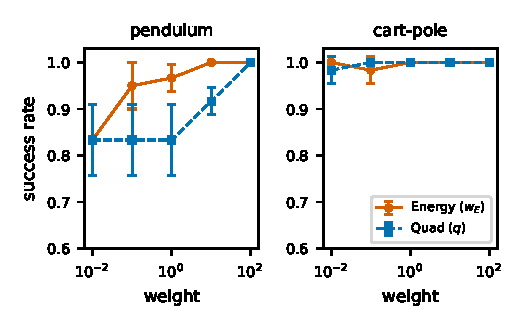
\includegraphics[width=\columnwidth]{sweep_success.pdf}\caption{Success rate vs.\ the swept weight ($w_E$ for iLQR-Energy, $q$ for iLQR-Quad), per task. Mean $\pm$ one sample std over 3 seeds, log $x$-axis.}\label{fig:swsr}\end{figure}
\begin{figure}[t]\centering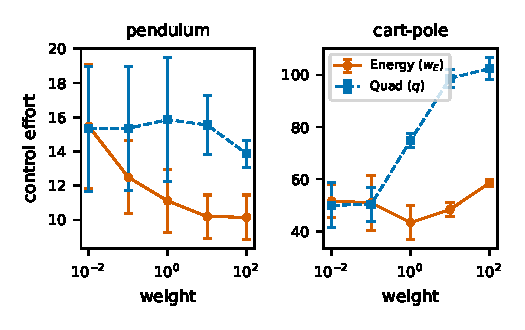
\includegraphics[width=\columnwidth]{sweep_effort.pdf}\caption{Control effort vs.\ the swept weight, per task. Mean $\pm$ one sample std over 3 seeds, log $x$-axis.}\label{fig:sweff}\end{figure}

\textbf{H3 (less sensitive to weight): refuted.} The registered test is the spread of the success rate across weights, and it is the same for the two costs on each task: across the five weights the mean success runs from \rhval{sweep_we/ilqr-energy-ours@we=0.01/pendulum/success_rate/mean:2} to \rhval{sweep_we/ilqr-energy-ours@we=100/pendulum/success_rate/mean:2} for the energy cost and from \rhval{sweep_qscale/ilqr-quad@qscale=0.01/pendulum/success_rate/mean:2} to \rhval{sweep_qscale/ilqr-quad@qscale=100/pendulum/success_rate/mean:2} for the quadratic cost on the pendulum, and from \rhval{sweep_we/ilqr-energy-ours@we=0.1/cartpole/success_rate/mean:2} to \rhval{sweep_we/ilqr-energy-ours@we=100/cartpole/success_rate/mean:2} and from \rhval{sweep_qscale/ilqr-quad@qscale=0.01/cartpole/success_rate/mean:2} to \rhval{sweep_qscale/ilqr-quad@qscale=100/cartpole/success_rate/mean:2} on the cart-pole. Effort tells a mixed story: the energy cost's effort varies more than the quadratic cost's on the pendulum (lowest to highest mean \rhval{sweep_we/ilqr-energy-ours@we=100/pendulum/control_effort/mean:1} to \rhval{sweep_we/ilqr-energy-ours@we=0.01/pendulum/control_effort/mean:1} vs \rhval{sweep_qscale/ilqr-quad@qscale=100/pendulum/control_effort/mean:1} to \rhval{sweep_qscale/ilqr-quad@qscale=1/pendulum/control_effort/mean:1}) and less on the cart-pole (\rhval{sweep_we/ilqr-energy-ours@we=1/cartpole/control_effort/mean:1} to \rhval{sweep_we/ilqr-energy-ours@we=100/cartpole/control_effort/mean:1} vs \rhval{sweep_qscale/ilqr-quad@qscale=0.01/cartpole/control_effort/mean:1} to \rhval{sweep_qscale/ilqr-quad@qscale=100/cartpole/control_effort/mean:1}). The two weights are not commensurable ($w_E$ multiplies a squared energy, $q$ a squared state error), so a ``same decade'' comparison is only indicative.

\textbf{Success depends on the weight.} Both costs improve with larger weights on the pendulum: $w_E\ge 10$ and $q=100$ give success \rhval{sweep_we/ilqr-energy-ours@we=10/pendulum/success_rate/mean:2} in the 3 seeds, above the default-weight values. With the best swept weight iLQR-Quad is also at \rhval{sweep_qscale/ilqr-quad@qscale=100/pendulum/success_rate/mean:2}, which removes the H1 gap.

\textbf{Effort across the sweep.} Table~\ref{tab:paired} compares iLQR-Quad at every $q$ with iLQR-Energy at its default $w_E=1$, paired over seeds 0--2. On the pendulum the quadratic cost uses more effort at every $q$ (by \rhval{cmp/pair_q100/ilqr-energy-ours/pendulum/control_effort/delta:1} to \rhval{cmp/pair_q1/ilqr-energy-ours/pendulum/control_effort/delta:1}). On the cart-pole the difference is \rhval{cmp/pair_q1/ilqr-energy-ours/cartpole/control_effort/delta:1} at the default $q=1$ and \rhval{cmp/pair_q10/ilqr-energy-ours/cartpole/control_effort/delta:1} to \rhval{cmp/pair_q100/ilqr-energy-ours/cartpole/control_effort/delta:1} for larger $q$, but only \rhval{cmp/pair_q0.01/ilqr-energy-ours/cartpole/control_effort/delta:1} and \rhval{cmp/pair_q0.1/ilqr-energy-ours/cartpole/control_effort/delta:1} for $q=0.01$ and $q=0.1$, with paired $p$ of \rhval{cmp/pair_q0.01/ilqr-energy-ours/cartpole/control_effort/paired_p:3} and \rhval{cmp/pair_q0.1/ilqr-energy-ours/cartpole/control_effort/paired_p:3} at $n=3$. The reverse reading matters too: iLQR-Energy at $w_E=0.01$, 0.1 and 100 (\rhval{sweep_we/ilqr-energy-ours@we=0.01/cartpole/control_effort/mean:1}, \rhval{sweep_we/ilqr-energy-ours@we=0.1/cartpole/control_effort/mean:1}, \rhval{sweep_we/ilqr-energy-ours@we=100/cartpole/control_effort/mean:1}) is not below iLQR-Quad at $q\le 0.1$ (\rhval{sweep_qscale/ilqr-quad@qscale=0.01/cartpole/control_effort/mean:1}, \rhval{sweep_qscale/ilqr-quad@qscale=0.1/cartpole/control_effort/mean:1}). So on the cart-pole the energy cost is nominally cheaper than the re-weighted quadratic cost only at $w_E=1$ and $w_E=10$ (\rhval{sweep_we/ilqr-energy-ours@we=1/cartpole/control_effort/mean:1} and \rhval{sweep_we/ilqr-energy-ours@we=10/cartpole/control_effort/mean:1}), by a margin that 3 seeds do not clearly resolve.

\begin{table}[t]\centering\caption{Effort of iLQR-Quad at each $q$ minus effort of iLQR-Energy at $w_E=1$ ($\Delta$ effort, positive: energy cost is cheaper), paired $t$-test over seeds 0--2, and the success rate of iLQR-Quad at that $q$.}\label{tab:paired}
\setlength{\tabcolsep}{5pt}\begin{tabular}{llrrrrr}\toprule
Task & & $q{=}0.01$ & 0.1 & 1 & 10 & 100 \\\midrule
pend. & $\Delta$ effort & 4.2 & 4.2 & 4.7 & 4.4 & 2.8 \\
 & paired $p$ & 0.059 & 0.057 & 0.047 & $<$0.001 & 0.044 \\
 & Quad success & 0.83 & 0.83 & 0.83 & 0.92 & 1.00 \\
cart-p. & $\Delta$ effort & 6.7 & 6.9 & 31.5 & 55.4 & 59.1 \\
 & paired $p$ & 0.046 & 0.090 & 0.027 & 0.003 & 0.008 \\
 & Quad success & 0.98 & 1.00 & 1.00 & 1.00 & 1.00 \\
\bottomrule
\end{tabular}
\end{table}

\textbf{Tuned comparison.} To compare the costs at equal tuning budget we pick, for each cost and task, the swept weight with the highest mean success on seeds 0--2 (ties broken by lowest mean effort) and add seeds 3--4 at that weight (Table~\ref{tab:tuned}). This picks $w_E=100$ and $q=100$ on the pendulum, and $w_E=1$ and $q=0.1$ on the cart-pole. The rule was fixed after seeing the sweep, so this is a post-hoc analysis. Success is \rhval{tuned_all/ilqr-energy-ours/pendulum/success_rate/mean:2} vs \rhval{tuned_all/ilqr-quad/pendulum/success_rate/mean:2} on the pendulum and \rhval{tuned_all/ilqr-energy-ours/cartpole/success_rate/mean:2} vs \rhval{tuned_all/ilqr-quad/cartpole/success_rate/mean:2} on the cart-pole: no success advantage remains. Effort stays lower for the energy cost, \rhval{tuned_all/ilqr-energy-ours/pendulum/control_effort/mean:1} vs \rhval{tuned_all/ilqr-quad/pendulum/control_effort/mean:1} on the pendulum and \rhval{tuned_all/ilqr-energy-ours/cartpole/control_effort/mean:1} vs \rhval{tuned_all/ilqr-quad/cartpole/control_effort/mean:1} on the cart-pole (paired $p$ of \rhval{cmp/tuned_all/ilqr-energy-ours/pendulum/control_effort/paired_p:4} and \rhval{cmp/tuned_all/ilqr-energy-ours/cartpole/control_effort/paired_p:3} at $n=5$). The 5 seeds include the 3 used for selection, for both costs alike; on the two held-out seeds alone the means are \rhval{tuned/ilqr-energy-ours/pendulum/control_effort/mean:1} vs \rhval{tuned/ilqr-quad/pendulum/control_effort/mean:1} and \rhval{tuned/ilqr-energy-ours/cartpole/control_effort/mean:1} vs \rhval{tuned/ilqr-quad/cartpole/control_effort/mean:1}, with no test at $n=2$. Time to upright is not distinguishable (\rhval{tuned_all/ilqr-energy-ours/pendulum/time_to_upright/mean:2} vs \rhval{tuned_all/ilqr-quad/pendulum/time_to_upright/mean:2}\,s; \rhval{tuned_all/ilqr-energy-ours/cartpole/time_to_upright/mean:2} vs \rhval{tuned_all/ilqr-quad/cartpole/time_to_upright/mean:2}\,s). Only one weight per cost was tuned; $r$, $Q_f$ and the horizon were not.

\begin{table}[t]\centering\caption{Tuned comparison: each cost at the weight picked on seeds 0--2 (highest success, ties by lowest effort). Mean $\pm$ sample std over seeds 0--4; last column: mean effort on the held-out seeds 3--4 only. Paired $t$-test between the two costs over the 5 seeds (--: no variance).}\label{tab:tuned}
\setlength{\tabcolsep}{3.5pt}\begin{tabular}{llrrrr}\toprule
Task & Cost (weight) & success & effort & time (s) & eff.\ 3--4 \\\midrule
pend. & Energy ($w_E$=100) & 0.99$\pm$0.02 & 10.9$\pm$1.5 & 2.29$\pm$0.18 & 12.0 \\
pend. & Quad ($q$=100) & 1.00$\pm$0.00 & 14.4$\pm$1.2 & 2.26$\pm$0.15 & 15.3 \\
 & paired $p$ ($n{=}5$) & 0.374 & $<$0.001 & 0.374 & \\
\midrule
cart-p. & Energy ($w_E$=1) & 1.00$\pm$0.00 & 42.0$\pm$6.0 & 1.79$\pm$0.06 & 40.1 \\
cart-p. & Quad ($q$=0.1) & 1.00$\pm$0.00 & 48.6$\pm$5.5 & 1.75$\pm$0.08 & 46.2 \\
 & paired $p$ ($n{=}5$) & -- & 0.009 & 0.103 & \\
\bottomrule
\end{tabular}
\end{table}


\section{Limitations}\label{sec:limitations}
This is a small CPU study. Two low-dimensional, noiseless plants with a perfect model; 5 seeds of 20 starts each (3 seeds for sweeps), so statistical tests have little power and success rates sit at a ceiling on the cart-pole. All baselines are reimplemented by us, not taken from reference code, and the energy-shaping gains were fixed once, not tuned; a better-tuned Astr\"om--Furuta controller could change H4. The default MPC weights were set by hand, their a-priori status rests on an unlogged pilot, and the sweeps show that the default operating point is not the best one for either cost: the main-table ranking depends on the weights, and the large cart-pole effort gap in particular reflects the default $Q$. The tuned comparison tunes a single weight per cost on a five-point grid, selects on 3 of the 5 seeds it reports, has only 2 held-out seeds, and was designed after the sweep. The term-magnitude diagnostic does not isolate a mechanism. The hysteresis switch and the cart-pole shaping law are our own design choices. The energy cost for the cart-pole counts the pole energy only. Control limits are handled by clipping in the rollout, not inside the backward pass. No multiple-comparison correction is applied to the pairwise tests. Solve times were measured on a shared machine and are not reported as a result. A fuller study would add model mismatch and noise, other horizons, joint weight tuning with equal budgets per method on separate seeds, shooting-based MPC, a double pendulum, and more seeds.


\section{Conclusion}\label{sec:conclusion}
In a small controlled comparison at hand-set default weights, an energy-deviation running cost made iLQR-MPC swing-up more successful than the quadratic cost on the pendulum and cheaper in control effort on both plants. Most of that advantage is tied to the default quadratic weight. The success gap is absent on the cart-pole (ceiling) and disappears on the pendulum with a larger quadratic weight. The cart-pole effort gap shrinks from \rhval{main/ilqr-energy-ours/cartpole/control_effort/mean:2} vs \rhval{main/ilqr-quad/cartpole/control_effort/mean:2} at default weights to \rhval{tuned_all/ilqr-energy-ours/cartpole/control_effort/mean:1} vs \rhval{tuned_all/ilqr-quad/cartpole/control_effort/mean:1} when each cost uses its best swept weight; on the pendulum the tuned gap is \rhval{tuned_all/ilqr-energy-ours/pendulum/control_effort/mean:1} vs \rhval{tuned_all/ilqr-quad/pendulum/control_effort/mean:1}. A lower effort for the energy cost at its default or tuned weight is thus the one effect that kept its direction against every quadratic weight we tried. Its size is modest once the quadratic cost is re-weighted, it rests on 5 seeds, three of them shared with weight selection, and on the cart-pole it does not hold for every energy weight. The energy cost was no less sensitive to its weight, was indistinguishable from the combined cost on the pendulum, and did not beat energy shaping with LQR catch there (energy shaping used less effort). Testing the costs under model error, with jointly tuned weights on separate seeds and tuned baselines, is the natural next step.


\bibliographystyle{IEEEtran}
\bibliography{refs}

\end{document}
